\chapter{Introduction}
\section{Motivation}
The world wide web is a phenomenon of ever increasing dimension and integration into people's lives. In the beginning of 2019 roughly 4.3 Billion people had access to the internet which accounts for 56\% of the entire world population\footnote{https://www.internetworldstats.com/stats.htm\#links, accessed: 30.03.2019}. 
With more people being interconnected the amount of available and generated data simultaneously increases.\\
This data encompasses a broad spectrum. Especially human related publicly or unintentionally shared information of web-searches, blogs, chats, video games, online shops and social media platforms have caught the interest of big-data analysts \parencite{Wu2014}. Social media platforms provide services which allow users to create an online identity to present themselves to others by sharing personalised content. There are various social media platform providers available such as Facebook, Instagram, YouTube or Twitter to name a few - all with their specific target audience and descriptive upload content. This social media data is referred to as User Generated Content (UGC) or if it is georeferenced as Volunteered Geographic Information (VGI). This geo-tagged information as it is also known allows the mapping of data. It encompasses people's interests, performed activities, future intentions, sense-of-place and perception of locations \parencite{Goodchild2007}. The applications of this data range from business solution to predict consumer demand, product satisfaction or enterprise renown \parencite{Yang2019} to rumour propagation, topic evolution \parencite{Kazienko2015} as well as environmental applications such as spatial planing for outdoor recreation. Investigating the latter in conjunction with VGI will be the subject of interest to this thesis.\\
Recreation is an essential human need for good mental \parencite{Trenberth2002} and physical health. \textcite{Kaplan1960} was one of the earliest to study leisure. He identified among others the presence of a pleasant expectation and recollection as well as a psychological perception of freedom as important elements. According to \textcite{Dillard2011} there exist four types of values/motivations for leisure/recreation which are (1) escape (2) enhancing relationships (3) personal mastery and (4) winning. Nature in particular allows for escape and the experience of personal freedom through the mystery found in landscapes \parencite{Kaplan1989} where the mind can find clam and peace. \\
Activities that foster this mental state are also known among the terms nature-based recreation, outdoor recreation or soft ecotourism \parencite{Deng2002, Balmford2009} and are associated with e.g. cycling, hiking, horse riding and wildlife watching. The provision of nature-based recreation is considered to be a cultural ecosystem services \parencite{Weyland2014, Richards2018, Yoshimura2017} with potentially high monetary value. \textcite{Shrestha2007} showed with the travel-cost method that people were willing to pay on average \$74.18 per visiting-day for nature-based recreation in the Apalachicola River region of Florida. \\
The presented health benefits and the monetary value associated with nature-based recreation shall illustrate the importance of its spatial mapping. Knowing peoples' usage of space is needed to provide, secure and improve these services and the allocation of recreational infrastructure by spatial planning agencies \parencite{Sen2014}. The mapping process becomes increasingly important considering a growing land-use intensity through higher recreational demands which could lead to uncontrolled and excessive land encroachment, an increase in greenhouse gas emissions as well as light and noise pollution \parencite{Song2018}.
VGI from social media platforms that host geo-tagged images with attached user-generated text were proven to be good indicators for multiple similar applications such as determining visitation rates to nature reserves \parencite{Tenkanen2017, Heikinheimo2017, Keeler2015, Wood2013} or to social events \parencite{Pettersson2011}, human mobility patterns \parencite{Barchiesi2015, Grossenbacher2014} and recreational locations \parencite{Weyland2014, Hill2006, Neuvonen2010}. The main advantages of these approaches to conventional methods such as surveys and interviews are comparably fast, (mostly) easy and low-priced \parencite{Richards2018} continuous data-streams as well as a good spatial and temporal coverage at small \parencite{Buckee2015b} and coarse scales \parencite{Weyland2014}. \\
An additional motivation to investigate the potential of social media data as proxy for the spatial occurrences of nature-based recreational is given by the increased rates of job induced mental fatigue, stress and illness which are side products of an ever more specialised and demanding economy \parencite{Trenberth2002}. To address that issue the report of mental health in Switzerland \parencite{Ruesch2003} was conducted among others by the Federal Office for Public Health (FOPH) which highlights the lack of prevention measures in place. This led to a monitoring program to foster mental health provision and awareness in Switzerland \parencite{Schuler2012} also on a cantonal level. The environment is known to be a sustainable source for mental health benefits by providing a diverse range of recreation possibilities. The extent and potential value associated with these provided ecosystem-services was noted in the 'effects of the environment on human health' report \parencite{Ragettli2017} of the Federal Office for the Environment (FOEN).

%According to the Federal Statistical Office (FSO) of Switzerland 73\% of people between the age of 16 and 74 were in the year 2017 in the possession of a smart mobile device\footnote{https://www.bfs.admin.ch/bfs/de/home/statistiken/kultur-medien-informationsgesellschaft-sport/informationsgesellschaft/gesamtindikatoren/haushalte-bevoelkerung/mobile-internetnutzung.html, accessed: 30.03.2019}. These devices are generally equipped with the Global Positioning System (GPS) which supports the provision of VGI.
%This social media derived big-data holds a lot of potential for various research applications as already highlighted by papers such as \textcite{DiMinin2015, DiMinin2017, Meentemeyer2016}. The main advantages to conventional methods such as surveys and interviews are comparably fast, (mostly) easy and low-priced continuous data-streams as well as a good spatial and temporal coverage at small \parencite{Buckee2015b} and coarse scales \parencite{Weyland2014}.\\

%xxxxxMENTAL HEALTHxxxxx
%The importance of leisure as a means of coping with work related stress has been shown by \textcite{Trenberth2002}
%Also a phenomenon of modern times are increased rates of job induced mental fatigue, stress and illness which are side products of an ever more specialised and demanding economy. To address that issue the report of mental health in Switzerland \parencite{Ruesch2003} was conducted among others by the Federal Office for Public Health (FOPH) which highlights the lack of prevention measures in place. This led to a monitoring program to foster mental health provision and awareness in Switzerland \parencite{Schuler2012} also on a cantonal level. The environment is known to be a sustainable source for mental health benefits by providing a diverse range of recreation possibilities. The extent and potential value associated with these provided ecosystem-services was noted in the 'effects of the environment on human health' report \parencite{Ragettli2017} of the Federal Office for the Environment (FOEN). \\

\section{Problem statement and aim}
Identifying and mapping activities related to nature-based recreation, outdoor recreation or soft ecotourism is the aim of this thesis.
Increasing the quality, quantity and attractiveness of nature-based recreation requires knowledge over the current usage of space. More specifically, in regards to the activities people perform in the environment to answer the following questions: (1) What nature-based recreational activity (NBRA) should be promoted in a certain area and (2) what kind of supportive infrastructure should be constructed to maximise its utilisation? This thesis tries to respond to that current need for information by investigating the potential of social media data in particular from the social media platforms Instagram\footnote{https://www.instagram.com/} and Flickr\footnote{https://www.flickr.com/} for analysing and monitoring the spatial occurrences of recreational activities including walking, hiking, jogging, biking, dog walking, horse riding and picnicking in the Canton of Zug, Switzerland. The mentioned social media platforms are known for hosting VGI in the form of user-generated text together with geotagged images (for more detailed information refer to section \ref{data_acquisition}). Accordingly, this study aims to evaluate the potential of social media data as a proxy for predicting the occurrences of recreational activities as an alternative to conventional data-acquisition methods such as surveys and interviews.\\
The goal of comparing people's usage of space with already present infrastructure to evaluate an efficient asset allocation was performed with the data of the web-application Foursquare\footnote{https://de.foursquare.com/}. This data consists of categorised infrastructural elements also known as \textit{venues} which were used as indicator for the current dispersion of sport and recreational facilities in the research area. The results of this comparison have the potential to inform spatial planing by allowing to optimise the allocation of recreational infrastructure in correspondence to the where people actually recreate.

\section{Approach}
The approach presented in this thesis creates and evaluates two machine learning (ML) models to predict recreational activities in georeferenced Instagram and Flickr posts. These posts are referred to as media objects throughout the thesis. The first model is trained on a combination of text and image data which resembles a novel approach. The second model was solely trained on text data and functions as a baseline reference to investigate the effect of including image content information. Structural image elements are extracted with the help of a deep-learning algorithm named Google Cloud Vision as also used by \textcite{Richards2018}. The models are individually trained on 1'046 manually classified Instagram media objects originating from a dataset of the region of Zurich \parencite{Gruzd2016} and tuned for best performance. Classification specific model evaluations are subsequently manually conducted on the NBRA-predictions in the research area to compare the two finalised model performances based on untrained data.\\
The research area is located in the Canton of Zug and was chosen according to the authors existing spatial knowledge which helped to evaluate the models' predicted occurrences of recreational activities as well as choosing favourable locations for the ground truthing as explained further down. Additionally, Martina Brennecke from the spatial planning agency of the city of Zug was a known contact which allowed a fast consultation regarding potential areas of recreational interest. This resulted specifically in the perimeter for which Instagram data was acquired (see figure \ref{research_area}) that incorporates two overall concepts related to recreation in the Canton of Zug \parencite{BaudirektiondesKantonsZug2012, Berchtold2011}.\\
\newline
The innovation of this approach lies in the fully automated prediction process without any manual content analysis which uses predominantly openly accessible and free software. This approach allows reconstruction and application by potential users such as municipal authorities or agencies. \\
\newline
In the course of this thesis, additional ground truth data from interviews and passive observations was acquired in three locations within the research area. The interviews were used to gain insight on three topics. Firstly the drivers that motivate people to visit certain locations above others. Secondly the social media usage of the interviewees in terms of social media platform engagement, upload-frequency and behaviour. Lastly some personal details were recorded which were kept anonymous to gain information about the demographics of social media users. The passive observation as second part of the ground truth was used to count NBRA-occurrences during the time the interviews were held. Recreational activity specific frequencies, locational visitation motivations and dominantly used social media platforms were among others derived signals from the ground truthing which were eventually compared to the social media data to evaluate the ML models.

\section{Background of machine learning}
This section provides a short introduction into the field of machine learning (ML) as well as a basic understanding of associated terminologies. The knowledge about ML was predominantly drawn from the book "Introduction to Machine Learning with Python" by \textcite{Guido2016}. The book covers the basic up to advanced concepts of ML and is recommended for further reference.\\
ML in its core refers to the process of a computer to understand or 'learn' the relationships inside a dataset with the help of algorithms to be able to make predictions on data the model has never seen before.
The training data normally consists of different features which identify and characterise the relationship between the input (independent) and the output (dependant) variable. The combination of feature-values which can be metaphorical seen as a 'fingerprint' of a given data point are the reason why a model can potentially make out patterns and relate them to a certain output. This output can either be a class (in the case of a classification problem) or a continuous number (in the case of a regression problem) of new data point.
An example of potential features of a regression problem could be different body measurements of a specific animal with the aim to differentiate between different types of the same species. The training data would then consist of multiple instances where most likely a human measured the needed body parts of several individuals and entered the continuous numerical value in the corresponding feature field.\\
\newline
There are two types of ML models - supervised and unsupervised learning. To illustrate the difference imagine a set of training data where each entry is represented by a point in an n-dimensional space where \textit{n} corresponds to the number of features present and the coordinates of each point (position vector of that point) correspond to the feature values. If we make the link back to the example above then unsupervised learning would mean that the training data consists of only the training data without any labels. The labels in this case would have been the names of the animal species that the measurements were taken from. In this way the model is forced to find natural breaks / boundaries on its own in the training data by clustering similar data points together and regarding them as an independent class. The hypothesis here is that points closer to each other in space are more related to one another than distant ones - similar to the first law of geography. These model given class names do not correspond in any way to the actual names of the animals because the model has no information on it what so ever. It is up to the user to appropriately label the clusters / classes the model isolated.

\begin{figure}[h]
   \centering
   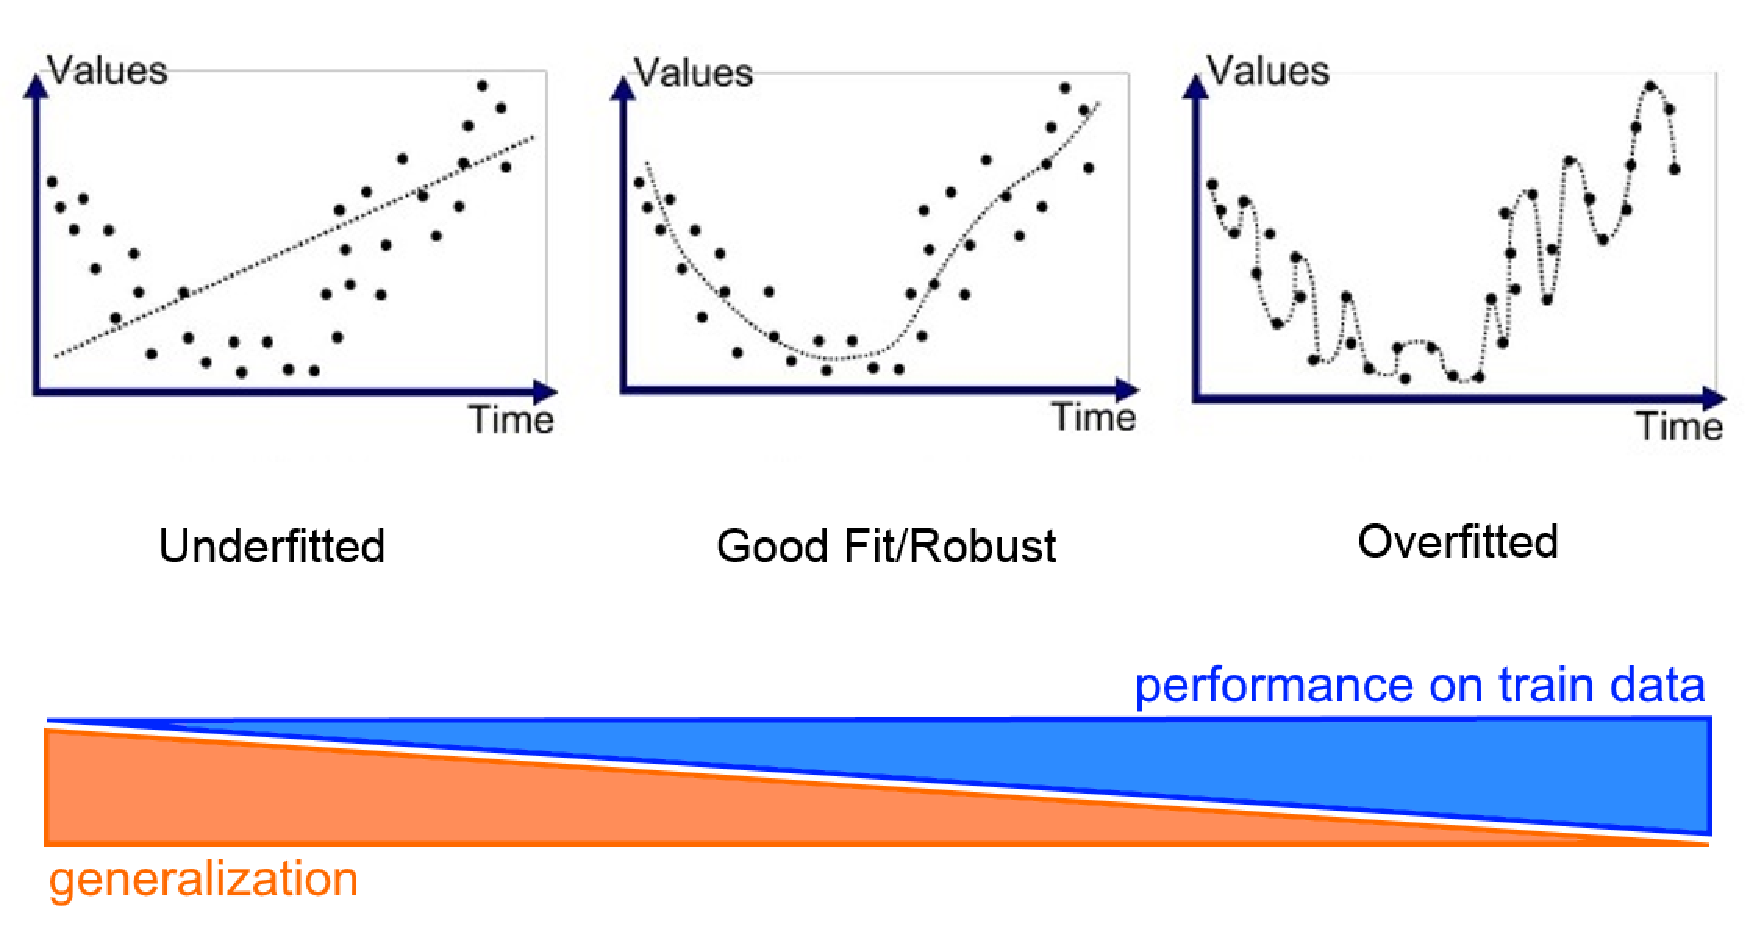
\includegraphics[width=0.9\textwidth]{img/over_underfitting}
   \caption{Visualisation of under- and overfitting on a dataset. Source: altered by the author, https://medium.com/greyatom/what-is-underfitting-and-overfitting-in-machine-learning-and-how-to-deal-with-it-6803a989c76, accessed: 29.03.2019}
   \label{fig:over_underfitting}
\end{figure}

Supervised learning on the other hand happens when the model is fed and trained upon example data with their correct classification labels present. The term 'supervised' therefore relates to the fact that presumably a human told the model which data points belong to which class. This approach is understandably more laborious because the creation of a labelled training dataset takes time. The benefits are generally better performing models and the possibility to directly validate and test the model. The difference between validation and testing becomes apparent in the three steps to finalise a model. To evaluate the most optimal ML algorithm for a use case they must first be fitted during the training phase on example-data where input is paired with expected output. Consecutively, the hyperparameters of the algorithm (see section \ref{model_setup}) are adjusted in the tuning phase on a specific validation set to yield the best performance. For a meaningful model validation a concept named k-fold cross-validation is often applied. Training and validation data are merged and the dataset is split into k folds. The model is now trained k times and every time a different subsets of the data is used for training and validation which results in more sophisticated model tuning. \\
Finally, the performance of the finalised, fully-trained model is evaluated on the test-set which was not used during model training nor model validation. If the size of the training data is big enough this separation into three parts is advised since "the test set error of the final chose model will underestimate the true test error, sometimes significantly" \parencite[p.222]{Hastie2017}. Otherwise, if the training dataset is small, common practise \parencite{Guido2016} is to split the original training dataset into a bigger portion ($\sim$ 75\%) for training and a smaller one ($\sim$ 25\%) for testing, neglecting the validation set. \\
\newline
Frequently used terms in relation to ML are under- and overfitting. These terms correspond to two extremes of how the model and its incorporated (boundary-) function is fitted to the provided test-data (see points in figure \ref{fig:over_underfitting}). Underfitting describes the state, where the model does not seem to extract and comprehend any logic from the dataset and therefore over-generalises the classification or regression problem at hand (see outer left graph of figure \ref{fig:over_underfitting}). \\
The other extreme is known by the term overfitting where the model tries to correctly classify every single training data point to its proper class. This results in the model being extremely tuned to the provided training data and its incorporated noise but not being able to generalise well on new unseen data (see outer right graph in figure \ref{fig:over_underfitting}). In other words overfitting basically means that the model tries to fit the training data so well that it lacks the generalisation ability on unseen data. The process of finding the balance between a model that is able to generalise on new data while identifying the underlying data-patterns is further described in section \ref{ml_text_data}.







